%%%%%%%%%%%%%%%%%%%%%%%%%%%%%%%%%%%%%%%%%%%%%%%%%%%%%%%%%%%%%%%%%%%%%%
% Overleaf (WriteLaTeX) Example: Molecular Chemistry Presentation
%
% Source: http://www.overleaf.com
%
% In these slides we show how Overleaf can be used with standard
% chemistry packages to easily create professional presentations.
%
% Feel free to distribute this example, but please keep the referral
% to overleaf.com
%
%%%%%%%%%%%%%%%%%%%%%%%%%%%%%%%%%%%%%%%%%%%%%%%%%%%%%%%%%%%%%%%%%%%%%%

\documentclass[xcolor={dvipsnames}]{beamer}

\mode<presentation>
{
  \usetheme{Madrid}       % or try default, Darmstadt, Warsaw, ...
  \usecolortheme{default} % or try albatross, beaver, crane, ...
  \usefonttheme{default}    % or try default, structurebold, ...
  \setbeamertemplate{navigation symbols}{}
  \setbeamertemplate{caption}[numbered]
}

\usepackage[english]{babel}
\usepackage[utf8x]{inputenc}
\usepackage{graphicx}
\usepackage{hyperref}
  \hypersetup{colorlinks=true}
  \hypersetup{urlcolor=blue}
  \hypersetup{linkcolor = .}
\usepackage{xcolor}
\usepackage{siunitx}
  \sisetup{separate-uncertainty = true}
\DeclareSIUnit\barn{b}
\usepackage{physics}
\usepackage[font=small,labelfont=bf]{caption}
\usepackage{subcaption}
\usepackage[en-GB]{datetime2}
\usepackage{overpic}
\usepackage{feynmp}
\DeclareGraphicsRule{*}{mps}{*}{}
\usepackage{scalerel}
\newcommand{\mylbrace}[2]{\vspace{#2pt}\hspace{6pt}\scaleleftright[\dimexpr5pt+#1\dimexpr0.06pt]{\lbrace}{\rule[\dimexpr2pt-#1\dimexpr0.5pt]{-4pt}{#1pt}}{.}}
\newcommand{\myrbrace}[2]{\vspace{#2pt}\scaleleftright[\dimexpr5pt+#1\dimexpr0.06pt]{.}{\rule[\dimexpr2pt-#1\dimexpr0.5pt]{-4pt}{#1pt}}{\rbrace}\hspace{6pt}}

% Trim in percent
\usepackage{adjustbox}

% No "Figure" prefix
\setbeamertemplate{caption}{\raggedright\insertcaption\par}

% Nice decay amplitude diagrams
\usepackage{amsmath,amssymb,tikz-cd}

% Strike out text
\usepackage[normalem]{ulem}

% For figures with text overlay
\usepackage{overpic}

% Arrows
\usepackage{tikz}
\newcommand{\tikzmark}[1]{\tikz[remember picture] \node[coordinate] (#1) {#1};}

% Colourbox with line breaks
\newcommand{\cbox}[2][lime!20]{%
  \colorbox{#1}{\parbox{\dimexpr\linewidth-2\fboxsep}{\strut #2\strut}}%
}

% Vector arrows
\usepackage[pdftex]{pict2e}

% Checkmark symbol
\def\checkmark{\tikz\fill[scale=0.4](0,.35) -- (.25,0) -- (1,.7) -- (.25,.15) -- cycle;}

% Here's where the presentation starts, with the info for the title slide
\title[Tracking efficiency meeting]{Update on 2025 post-TS tracking efficiencies}

\author[Martin Tat]{Martin Tat}
\institute[Heidelberg]{Heidelberg University}
\date{16th June 2026}

\titlegraphic{
\includegraphics[height = 2.3cm]{lhcb.jpg}\hspace{1.0cm}~%
              
\includegraphics[height = 2.3cm]{HeidelbergLogo.pdf}}

\begin{document}

\begin{frame}
  \titlepage
\end{frame}

% These three lines create an automatically generated table of contents.
%\begin{frame}{Outline}
%  \tableofcontents
%\end{frame}

\begin{frame}{Progress update}
  \vspace{0.0cm}
  {\large Progress update:}
  \vspace{0.2cm}
  \begin{enumerate}
    \setlength\itemsep{0.8em}
    \item{Tracking efficiency tables presented in RTA WP4 two weeks ago}
    \begin{itemize}
      \item[-]{No objections or issues raised}
      \item[-]{Tables pushed to GitLab repo for analysts to use on 4th June}
    \end{itemize}
    \item{Today: 2025 post-TS tables}
    \begin{itemize}
      \item[-]{MC request with priority 1a finished very quickly}
      \item[-]{Most fits converged without issues}
      \item[-]{I would like to release these tables as well}
    \end{itemize}
    \item{Plan to present a quick update in RTA WP4 on Thursday}
  \end{enumerate}
\end{frame}

\begin{frame}{2025 tracking efficiencies}
  \vspace{0.0cm}
  {\large Comparison of tracking efficiencies in 2025 data blocks}
  \begin{figure}[htb]
    \centering
    \begin{subfigure}{0.5\textwidth}
      \centering
      
\includegraphics[width=1.0\textwidth]{Plots/trackeff_Data_VeloMuon_P_workdir_samples.pdf}
    \end{subfigure}%
    \begin{subfigure}{0.5\textwidth}
      \centering
      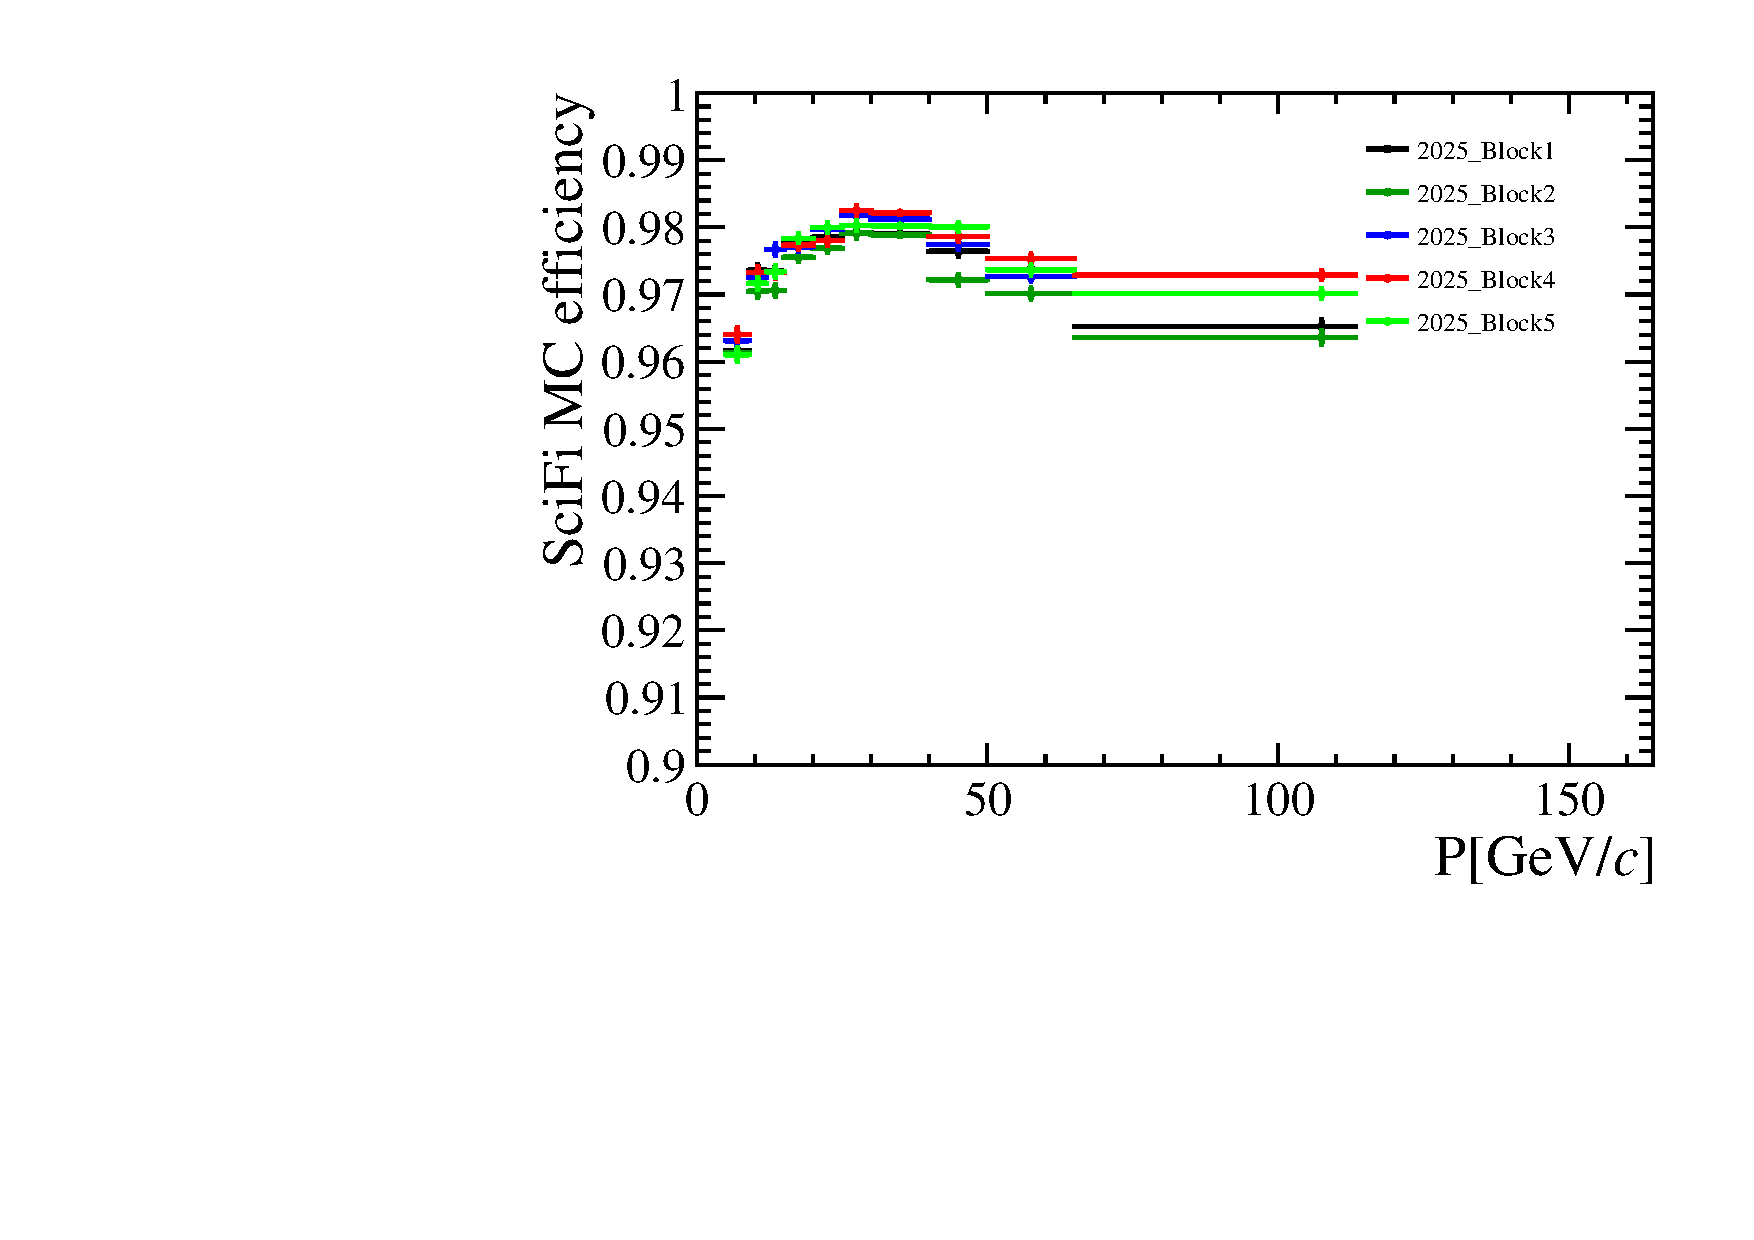
\includegraphics[width=1.0\textwidth]{Plots/trackeff_MC_VeloMuon_P_workdir_samples.pdf}
    \end{subfigure}
  \end{figure}
  {SciFi efficiencies dropping slowly over time in data}
\end{frame}

\begin{frame}{2025 tracking efficiencies}
  \vspace{0.0cm}
  {\large Comparison of tracking efficiencies in 2025 data blocks}
  \begin{figure}[htb]
    \centering
    \begin{subfigure}{0.5\textwidth}
      \centering
      
\includegraphics[width=1.0\textwidth]{Plots/trackeff_Data_VeloMuon_ETA_workdir_samples.pdf}
    \end{subfigure}%
    \begin{subfigure}{0.5\textwidth}
      \centering
      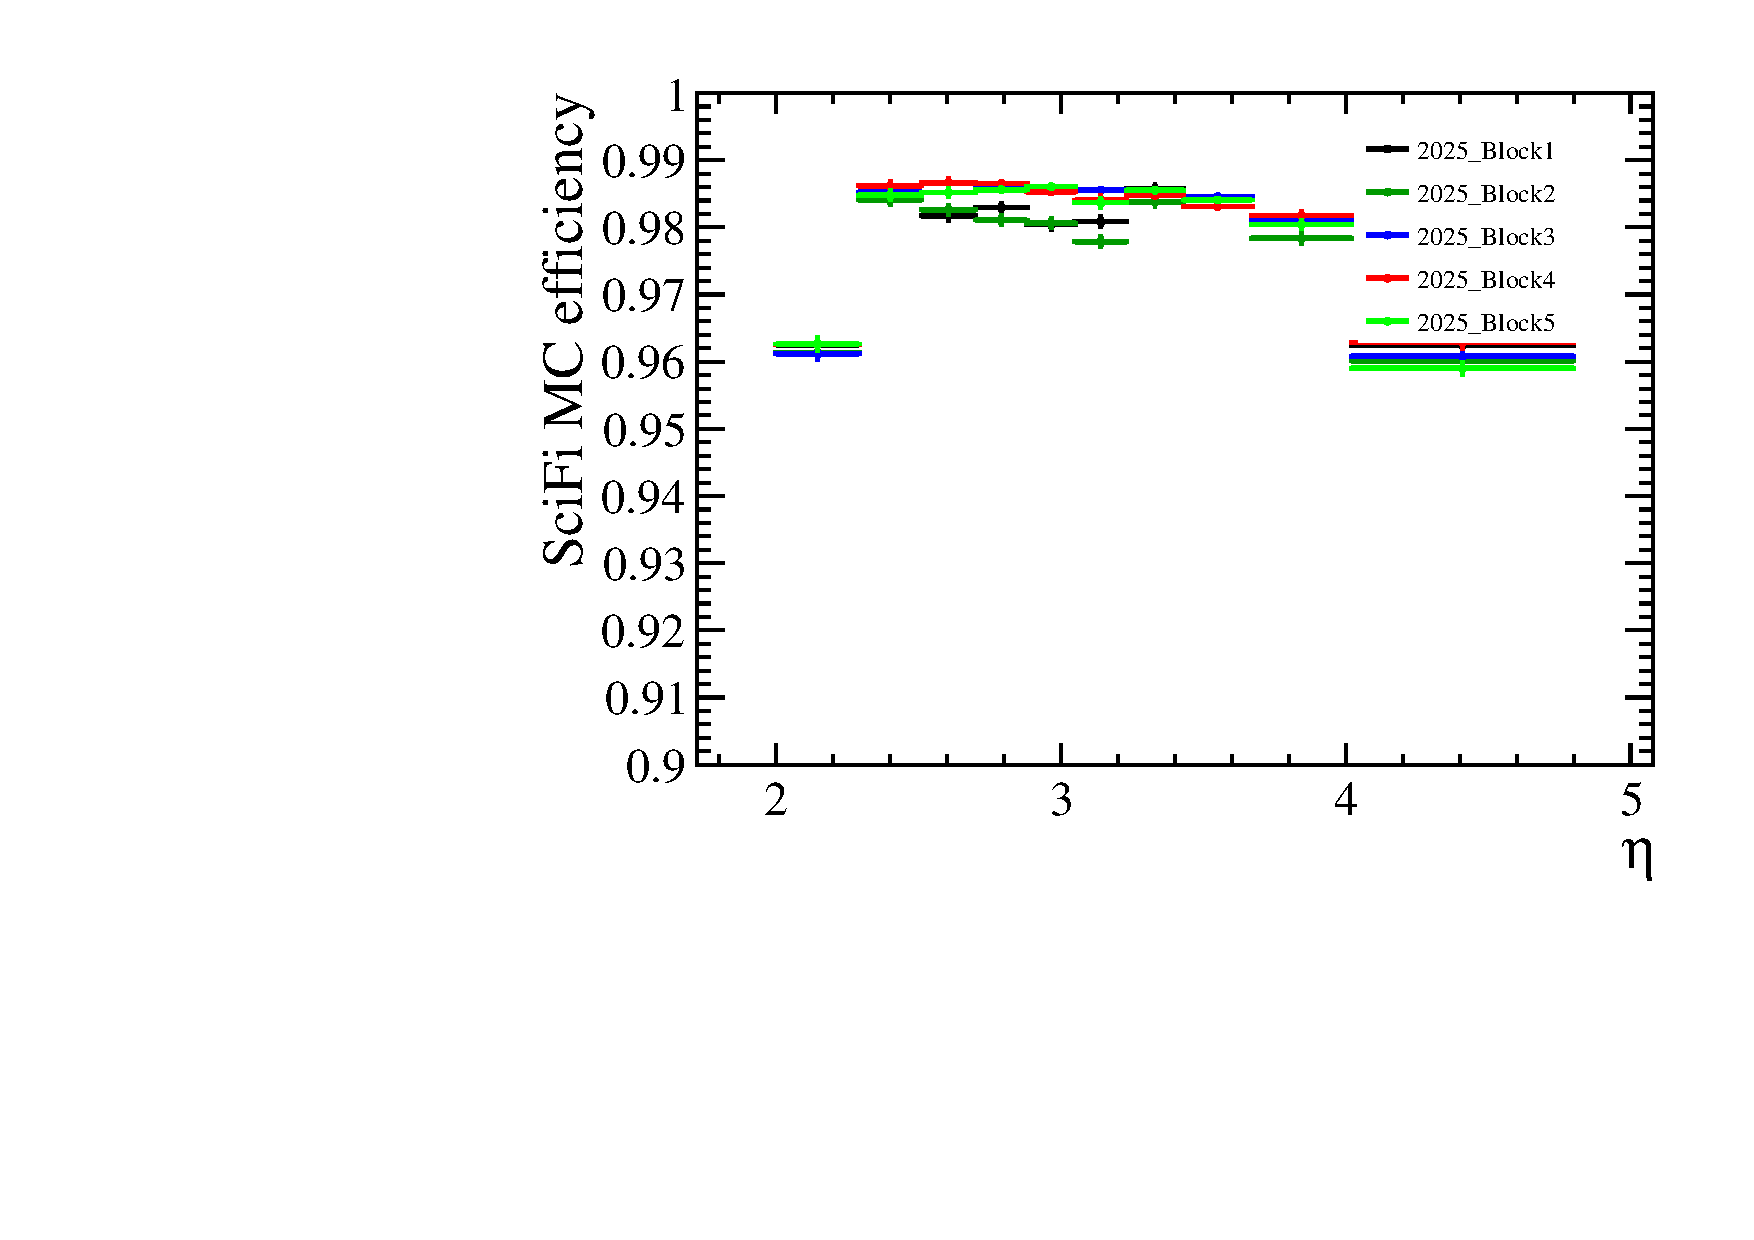
\includegraphics[width=1.0\textwidth]{Plots/trackeff_MC_VeloMuon_ETA_workdir_samples.pdf}
    \end{subfigure}
  \end{figure}
  {SciFi efficiencies dropping slowly over time in data}
\end{frame}

\begin{frame}{2025 tracking efficiencies}
  \vspace{0.0cm}
  {\large Comparison of tracking efficiencies in 2025 data blocks}
  \begin{figure}[htb]
    \centering
    \begin{subfigure}{0.5\textwidth}
      \centering
      
\includegraphics[width=1.0\textwidth]{Plots/trackeff_Data_Downstream_P_workdir_samples.pdf}
    \end{subfigure}%
    \begin{subfigure}{0.5\textwidth}
      \centering
      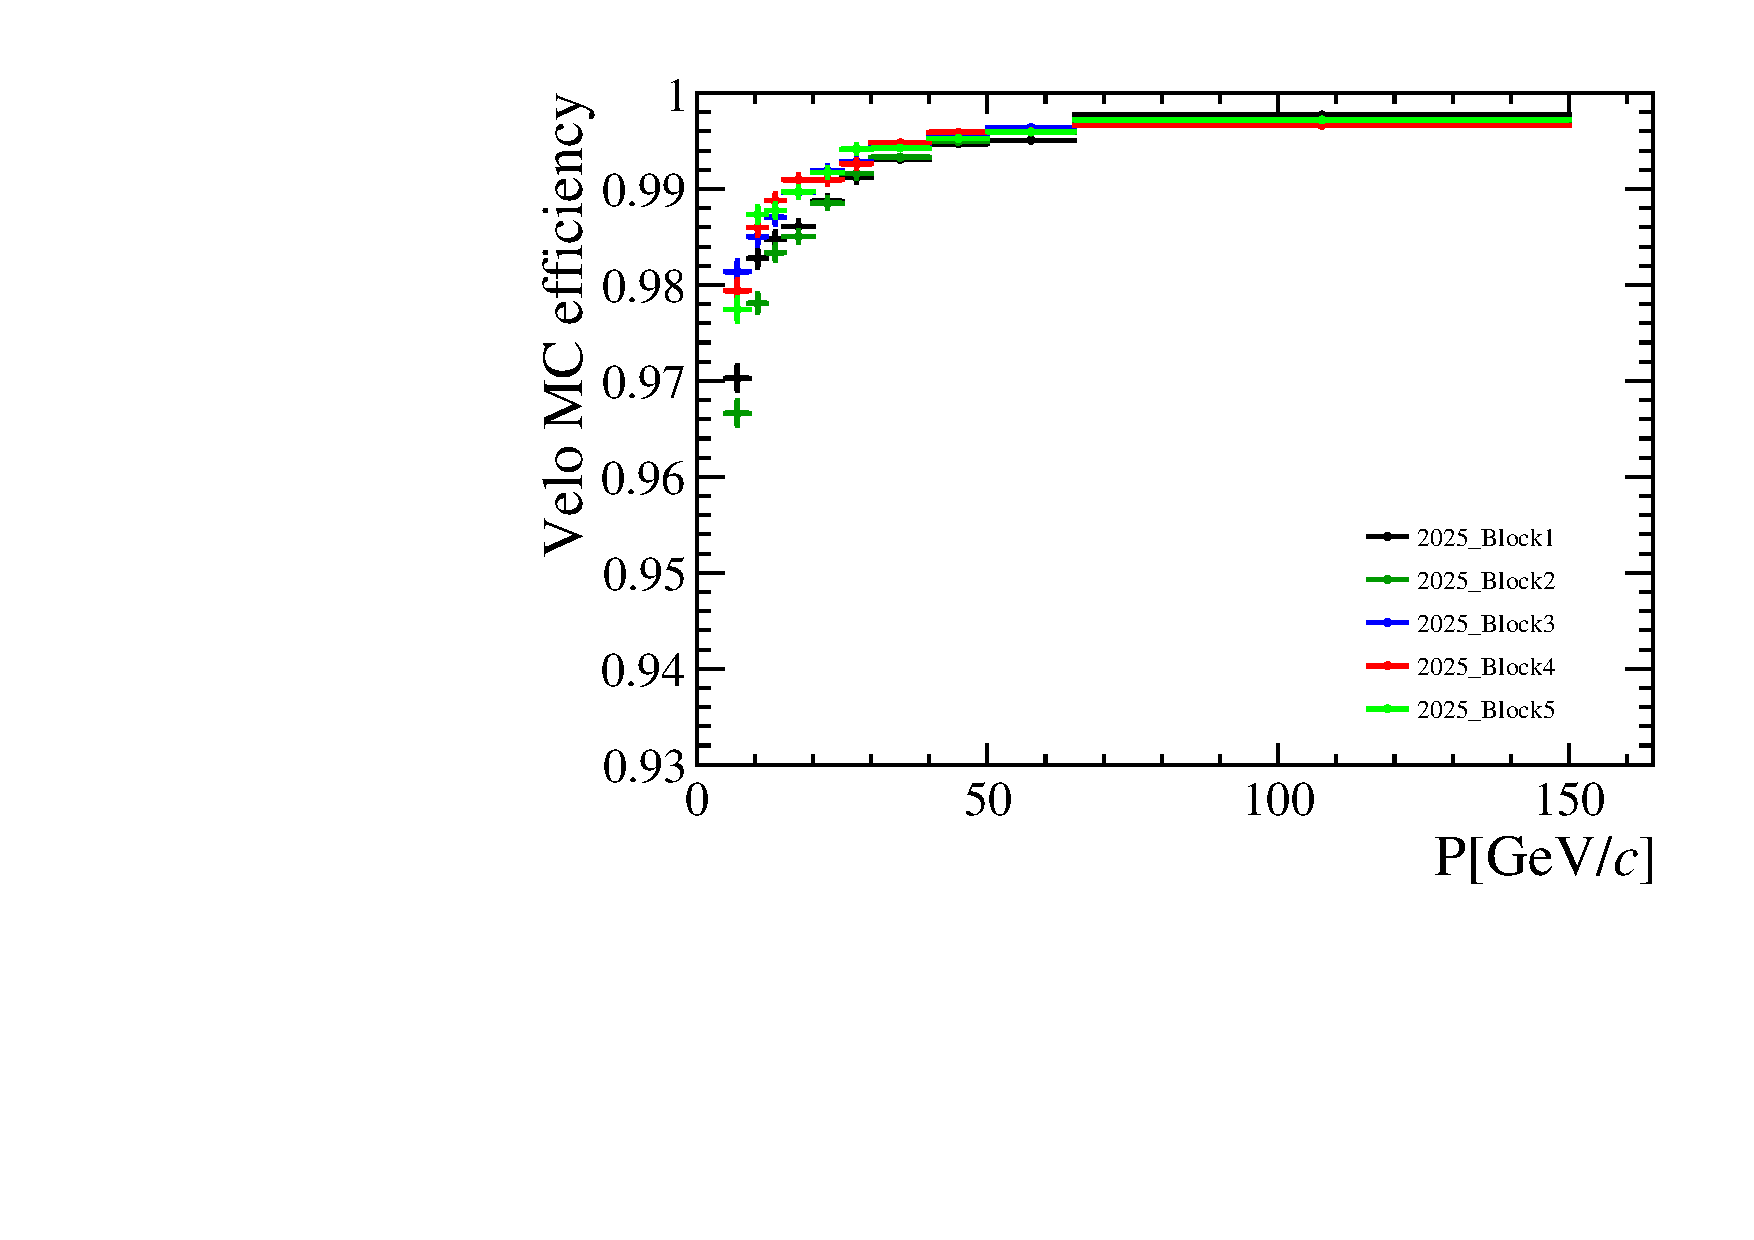
\includegraphics[width=1.0\textwidth]{Plots/trackeff_MC_Downstream_P_workdir_samples.pdf}
    \end{subfigure}
  \end{figure}
  {Velo efficiencies underestimated in blocks 1/2, but not blocks 3/4/5}
\end{frame}

\begin{frame}{2025 tracking efficiencies}
  \vspace{0.0cm}
  {\large Comparison of tracking efficiencies in 2025 data blocks}
  \begin{figure}[htb]
    \centering
    \begin{subfigure}{0.5\textwidth}
      \centering
      
\includegraphics[width=1.0\textwidth]{Plots/trackeff_Data_Downstream_ETA_workdir_samples.pdf}
    \end{subfigure}%
    \begin{subfigure}{0.5\textwidth}
      \centering
      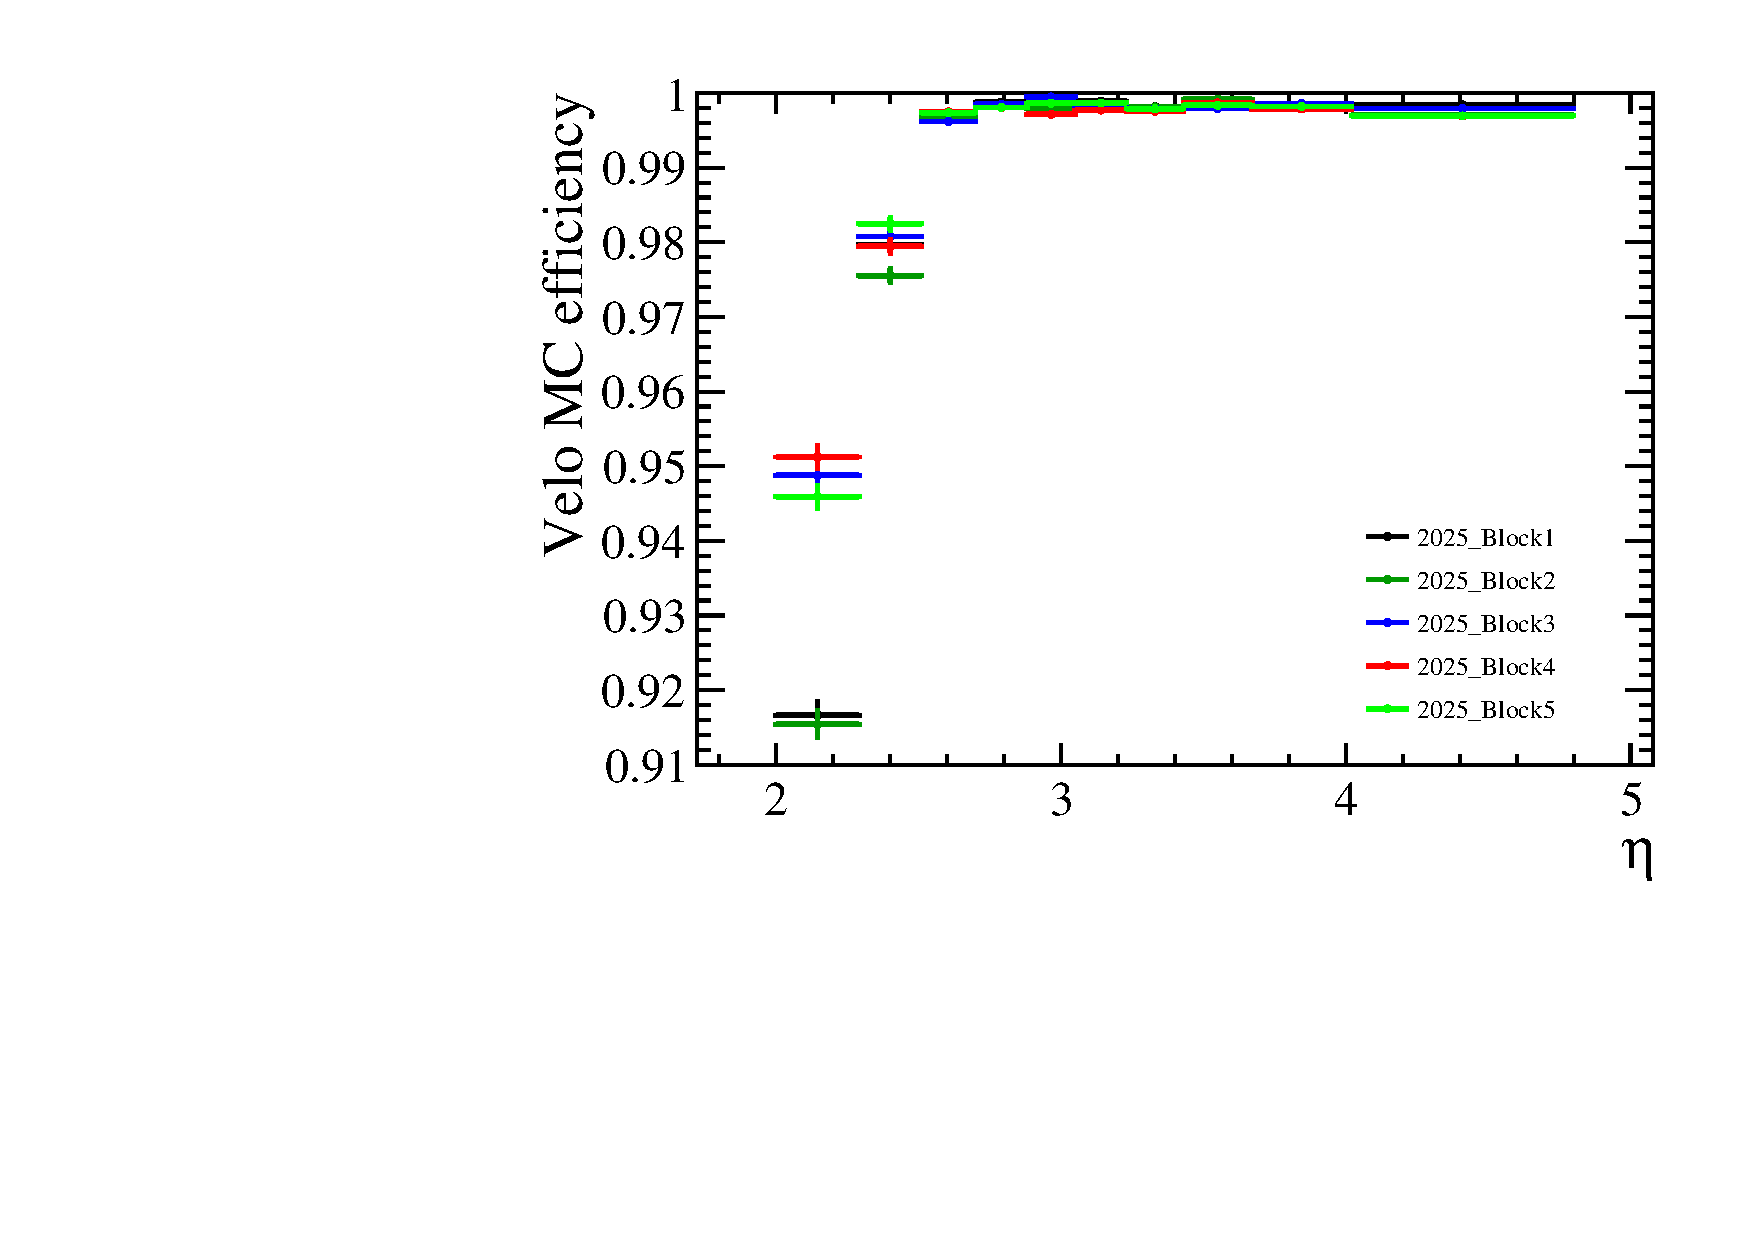
\includegraphics[width=1.0\textwidth]{Plots/trackeff_MC_Downstream_ETA_workdir_samples.pdf}
    \end{subfigure}
  \end{figure}
  {Velo efficiencies underestimated in blocks 1/2, but not blocks 3/4/5}
\end{frame}

\begin{frame}{2025 tracking efficiencies}
  \vspace{0.0cm}
  {\large Comparison of tracking efficiencies in 2025 data blocks}
  \begin{figure}[htb]
    \centering
    \begin{subfigure}{0.5\textwidth}
      \centering
      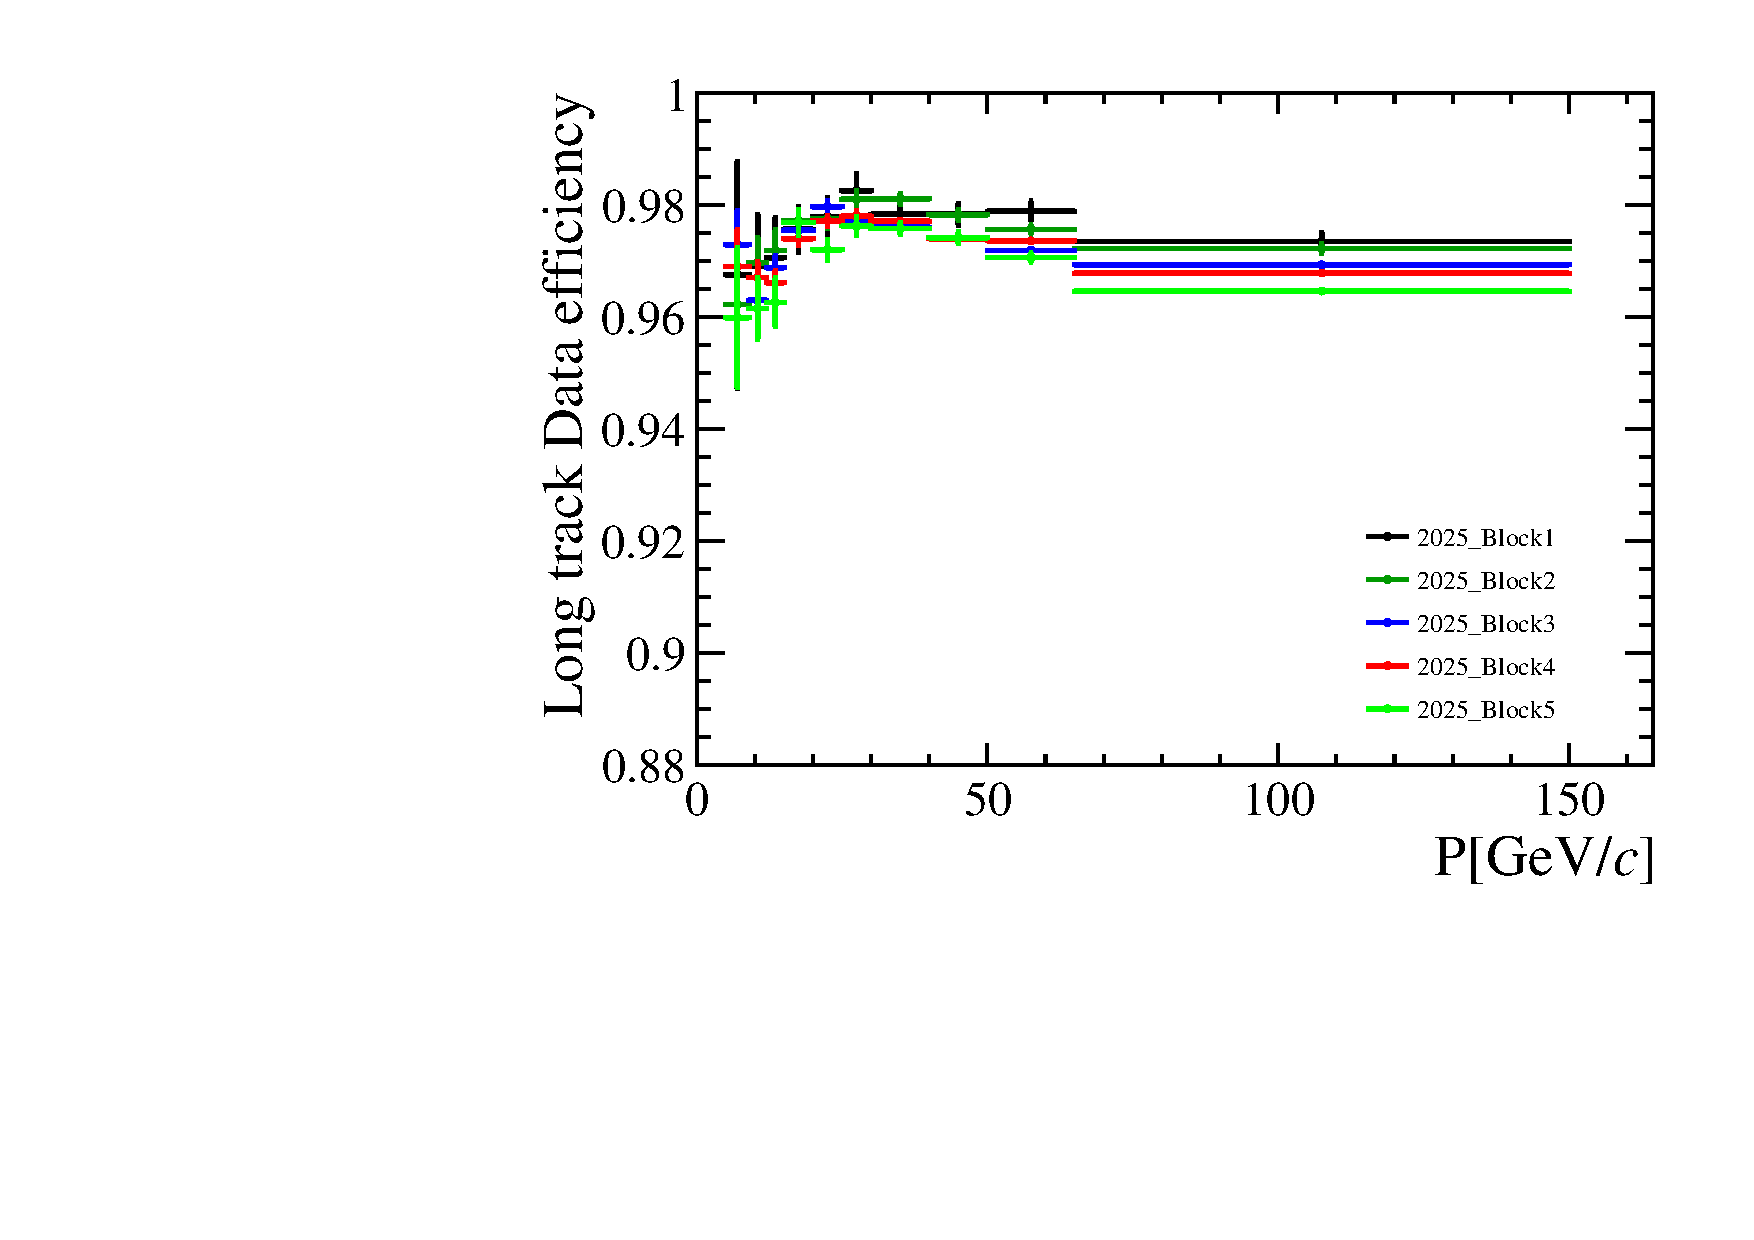
\includegraphics[width=1.0\textwidth]{Plots/trackeff_Data_MuonUT_P_workdir_samples.pdf}
    \end{subfigure}%
    \begin{subfigure}{0.5\textwidth}
      \centering
      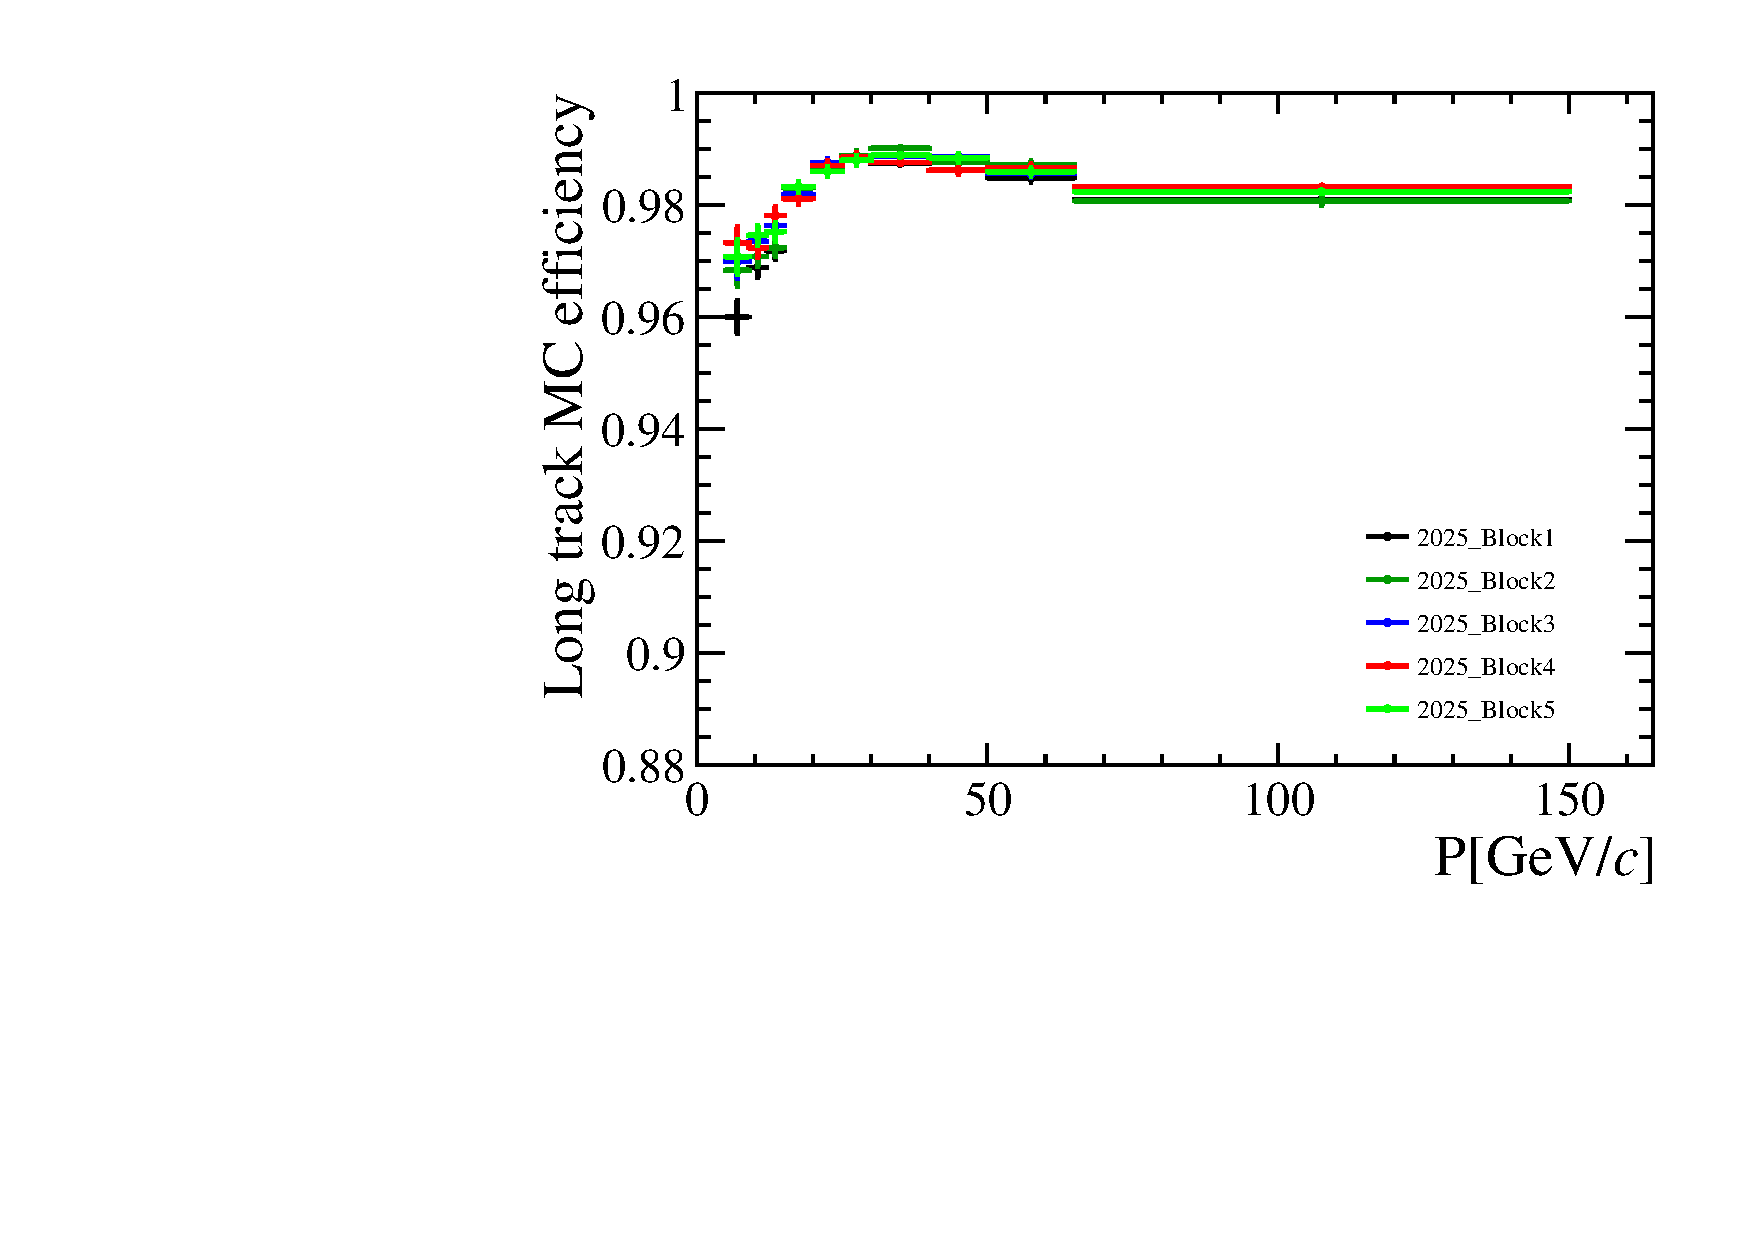
\includegraphics[width=1.0\textwidth]{Plots/trackeff_MC_MuonUT_P_workdir_samples.pdf}
    \end{subfigure}
  \end{figure}
  {MuonUT efficiencies look consistent, but lower statistics}
\end{frame}

\begin{frame}{2025 tracking efficiencies}
  \vspace{0.0cm}
  {\large Comparison of tracking efficiencies in 2025 data blocks}
  \begin{figure}[htb]
    \centering
    \begin{subfigure}{0.5\textwidth}
      \centering
      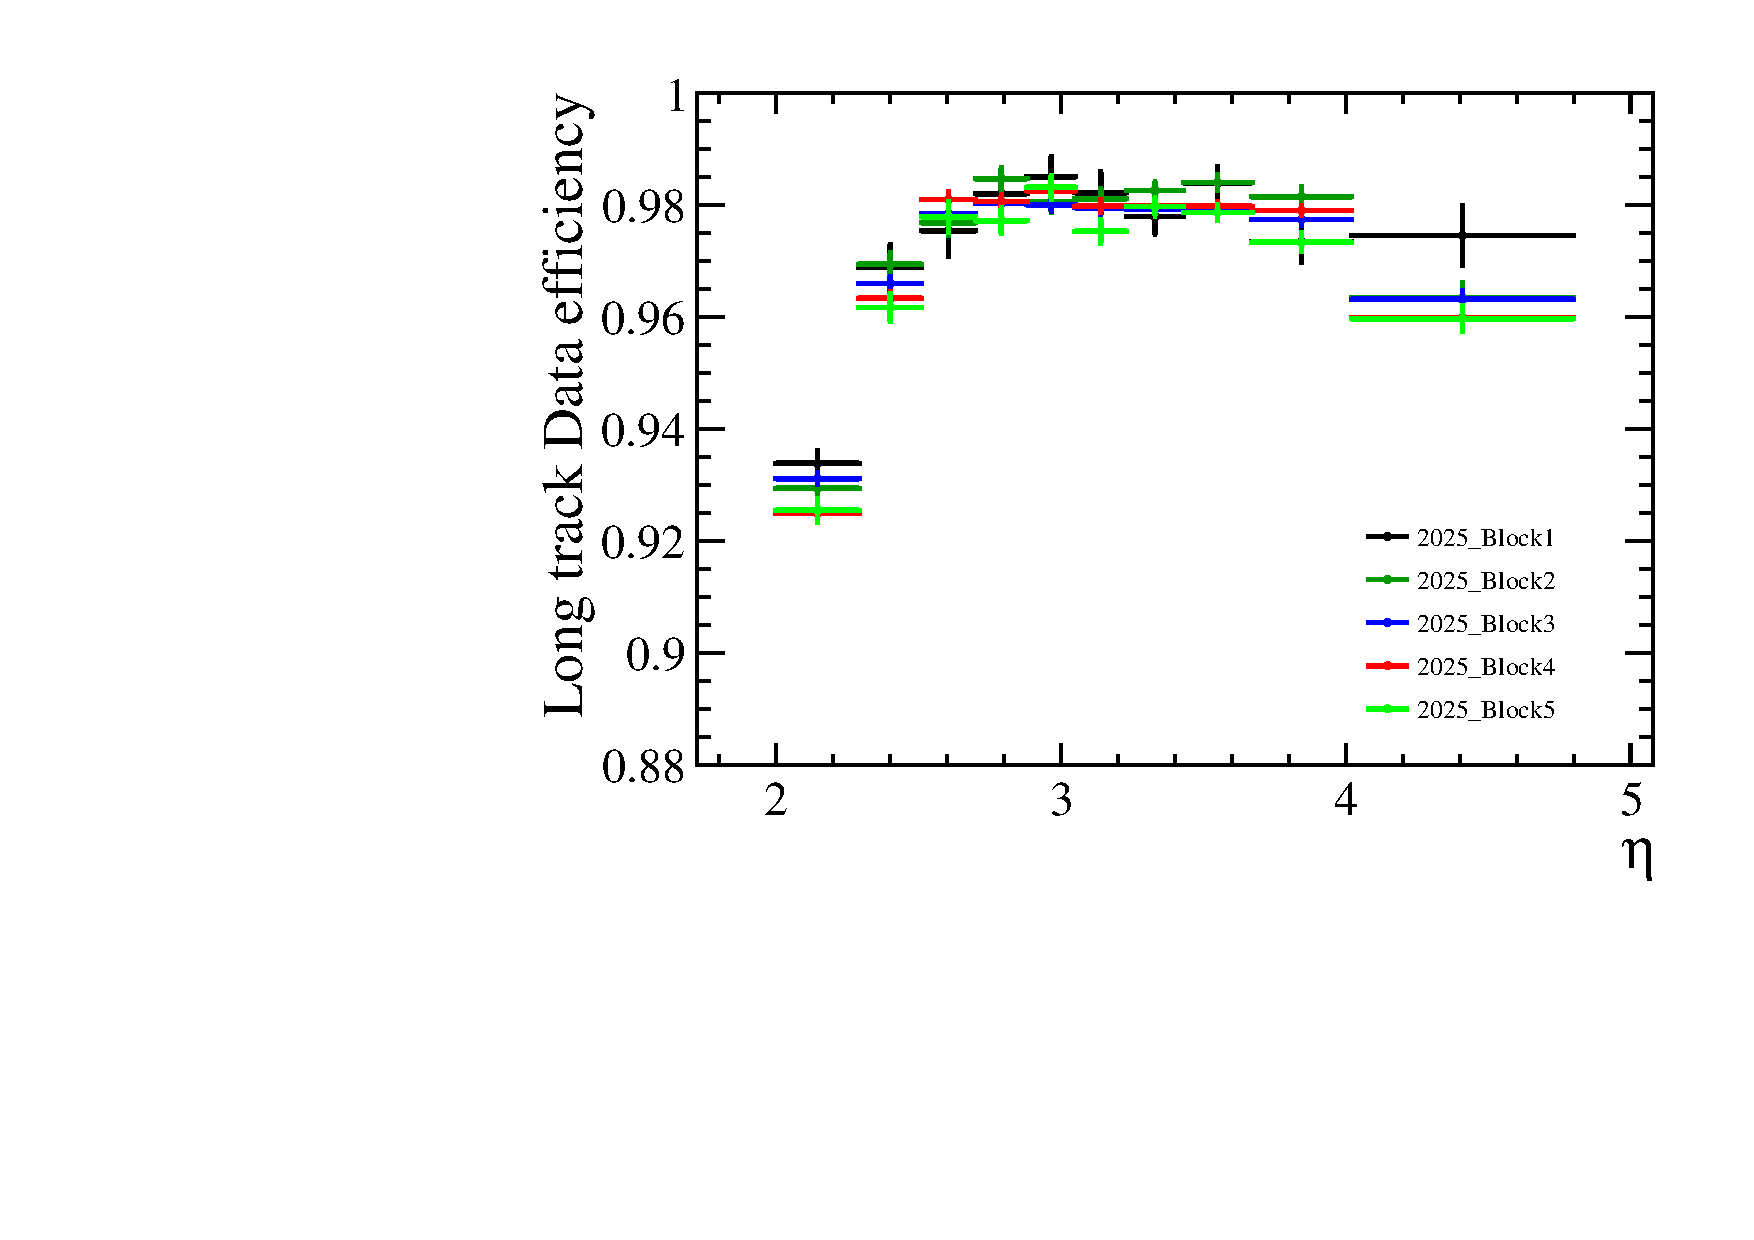
\includegraphics[width=1.0\textwidth]{Plots/trackeff_Data_MuonUT_ETA_workdir_samples.pdf}
    \end{subfigure}%
    \begin{subfigure}{0.5\textwidth}
      \centering
      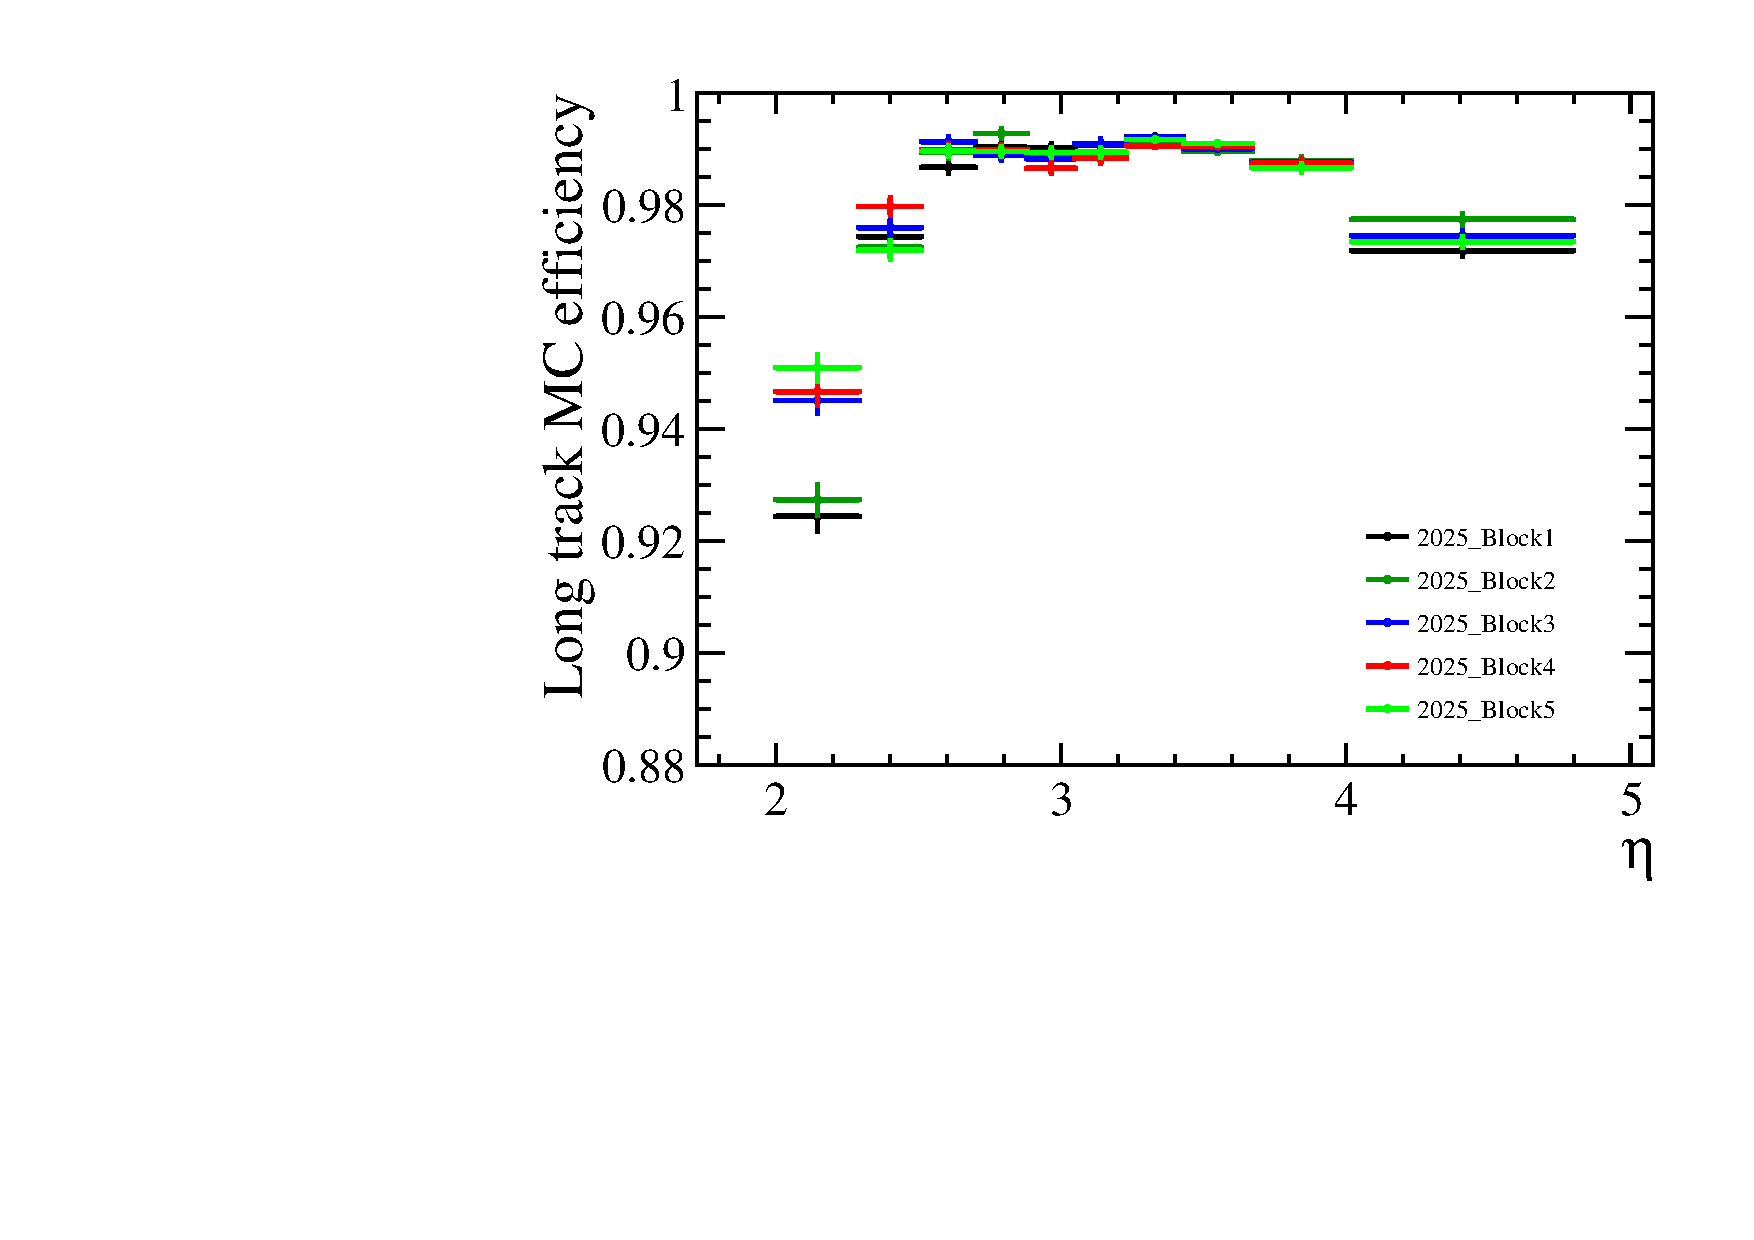
\includegraphics[width=1.0\textwidth]{Plots/trackeff_MC_MuonUT_ETA_workdir_samples.pdf}
    \end{subfigure}
  \end{figure}
  {MuonUT efficiencies look consistent, but lower statistics}
\end{frame}

\begin{frame}{2025 tracking efficiencies}
  \vspace{0.0cm}
  {\large Data-MC ratio in 2025 block 1}
  \begin{figure}[htb]
    \centering
    \begin{subfigure}{0.5\textwidth}
      \centering
      
\includegraphics[width=1.0\textwidth]{Plots/trackeff_ratio_P_2025_Block1_workdir_samples.pdf}
    \end{subfigure}%
    \begin{subfigure}{0.5\textwidth}
      \centering
      
\includegraphics[width=1.0\textwidth]{Plots/trackeff_ratio_ETA_2025_Block1_workdir_samples.pdf}
    \end{subfigure}
  \end{figure}
\end{frame}

\begin{frame}{2025 tracking efficiencies}
  \vspace{0.0cm}
  {\large Data-MC ratio in 2025 block 2}
  \begin{figure}[htb]
    \centering
    \begin{subfigure}{0.5\textwidth}
      \centering
      
\includegraphics[width=1.0\textwidth]{Plots/trackeff_ratio_P_2025_Block2_workdir_samples.pdf}
    \end{subfigure}%
    \begin{subfigure}{0.5\textwidth}
      \centering
      
\includegraphics[width=1.0\textwidth]{Plots/trackeff_ratio_ETA_2025_Block2_workdir_samples.pdf}
    \end{subfigure}
  \end{figure}
\end{frame}

\begin{frame}{2025 tracking efficiencies}
  \vspace{0.0cm}
  {\large Data-MC ratio in 2025 block 3}
  \begin{figure}[htb]
    \centering
    \begin{subfigure}{0.5\textwidth}
      \centering
      
\includegraphics[width=1.0\textwidth]{Plots/trackeff_ratio_P_2025_Block3_workdir_samples.pdf}
    \end{subfigure}%
    \begin{subfigure}{0.5\textwidth}
      \centering
      
\includegraphics[width=1.0\textwidth]{Plots/trackeff_ratio_ETA_2025_Block3_workdir_samples.pdf}
    \end{subfigure}
  \end{figure}
\end{frame}

\begin{frame}{2025 tracking efficiencies}
  \vspace{0.0cm}
  {\large Data-MC ratio in 2025 block 4}
  \begin{figure}[htb]
    \centering
    \begin{subfigure}{0.5\textwidth}
      \centering
      
\includegraphics[width=1.0\textwidth]{Plots/trackeff_ratio_P_2025_Block4_workdir_samples.pdf}
    \end{subfigure}%
    \begin{subfigure}{0.5\textwidth}
      \centering
      
\includegraphics[width=1.0\textwidth]{Plots/trackeff_ratio_ETA_2025_Block4_workdir_samples.pdf}
    \end{subfigure}
  \end{figure}
\end{frame}

\begin{frame}{2025 tracking efficiencies}
  \vspace{0.0cm}
  {\large Data-MC ratio in 2025 block 5}
  \begin{figure}[htb]
    \centering
    \begin{subfigure}{0.5\textwidth}
      \centering
      
\includegraphics[width=1.0\textwidth]{Plots/trackeff_ratio_P_2025_Block5_workdir_samples.pdf}
    \end{subfigure}%
    \begin{subfigure}{0.5\textwidth}
      \centering
      
\includegraphics[width=1.0\textwidth]{Plots/trackeff_ratio_ETA_2025_Block5_workdir_samples.pdf}
    \end{subfigure}
  \end{figure}
\end{frame}

\begin{frame}{2025 pre-TS tracking efficiency corrections}
  \vspace{0.0cm}
  \begin{figure}[htb]
    \centering
    
\includegraphics[width=0.85\textwidth]{Plots/TrackingEfficiencies_2D_binning_2025_Block3_Data_colour.pdf}
  \end{figure}
\end{frame}

\begin{frame}{2025 pre-TS tracking efficiency corrections}
  \vspace{0.0cm}
  \begin{figure}[htb]
    \centering
    
\includegraphics[width=0.85\textwidth]{Plots/TrackingEfficiencies_2D_binning_2025_Block3_MC_colour.pdf}
  \end{figure}
\end{frame}

\begin{frame}{2025 pre-TS tracking efficiency corrections}
  \vspace{0.0cm}
  \begin{figure}[htb]
    \centering
    
\includegraphics[width=0.85\textwidth]{Plots/TrackingEfficiencies_2D_binning_2025_Block3_Ratio_colour.pdf}
  \end{figure}
\end{frame}

\begin{frame}{2025 pre-TS tracking efficiency corrections}
  \vspace{0.0cm}
  \begin{figure}[htb]
    \centering
    
\includegraphics[width=0.85\textwidth]{Plots/TrackingEfficiencies_2D_binning_2025_Block3_RatioDiff_colour.pdf}
  \end{figure}
\end{frame}

\begin{frame}{2025 pre-TS tracking efficiency corrections}
  \vspace{0.0cm}
  \begin{figure}[htb]
    \centering
    
\includegraphics[width=0.85\textwidth]{Plots/TrackingEfficiencies_2D_binning_2025_Block4_Data_colour.pdf}
  \end{figure}
\end{frame}

\begin{frame}{2025 pre-TS tracking efficiency corrections}
  \vspace{0.0cm}
  \begin{figure}[htb]
    \centering
    
\includegraphics[width=0.85\textwidth]{Plots/TrackingEfficiencies_2D_binning_2025_Block4_MC_colour.pdf}
  \end{figure}
\end{frame}

\begin{frame}{2025 pre-TS tracking efficiency corrections}
  \vspace{0.0cm}
  \begin{figure}[htb]
    \centering
    
\includegraphics[width=0.85\textwidth]{Plots/TrackingEfficiencies_2D_binning_2025_Block4_Ratio_colour.pdf}
  \end{figure}
\end{frame}

\begin{frame}{2025 pre-TS tracking efficiency corrections}
  \vspace{0.0cm}
  \begin{figure}[htb]
    \centering
    
\includegraphics[width=0.85\textwidth]{Plots/TrackingEfficiencies_2D_binning_2025_Block4_RatioDiff_colour.pdf}
  \end{figure}
\end{frame}

\begin{frame}{2025 pre-TS tracking efficiency corrections}
  \vspace{0.0cm}
  \begin{figure}[htb]
    \centering
    
\includegraphics[width=0.85\textwidth]{Plots/TrackingEfficiencies_2D_binning_2025_Block5_Data_colour.pdf}
  \end{figure}
\end{frame}

\begin{frame}{2025 pre-TS tracking efficiency corrections}
  \vspace{0.0cm}
  \begin{figure}[htb]
    \centering
    
\includegraphics[width=0.85\textwidth]{Plots/TrackingEfficiencies_2D_binning_2025_Block5_MC_colour.pdf}
  \end{figure}
\end{frame}

\begin{frame}{2025 pre-TS tracking efficiency corrections}
  \vspace{0.0cm}
  \begin{figure}[htb]
    \centering
    
\includegraphics[width=0.85\textwidth]{Plots/TrackingEfficiencies_2D_binning_2025_Block5_Ratio_colour.pdf}
  \end{figure}
\end{frame}

\begin{frame}{2025 pre-TS tracking efficiency corrections}
  \vspace{0.0cm}
  \begin{figure}[htb]
    \centering
    
\includegraphics[width=0.85\textwidth]{Plots/TrackingEfficiencies_2D_binning_2025_Block5_RatioDiff_colour.pdf}
  \end{figure}
\end{frame}

\begin{frame}{Plan next}
  \vspace{0.0cm}
  {\large Next steps:}
  \vspace{0.2cm}
  \begin{enumerate}
    \setlength\itemsep{0.8em}
    \item{Large 2024 production is done}
    \begin{itemize}
      \item[-]{Produce v1 tables with $\mu^\pm$, $\mu^+$, $\mu^-$ using new binning, look into reweighting multiplicity}
      \item[-]{Will probably take a while, as I'm quite busy with analysis as well}
    \end{itemize}
    \item{Look into block 1b MC}
  \end{enumerate}
\end{frame}

\end{document}
